\documentclass{beamer}
%
% Choose how your presentation looks.
%
% For more themes, color themes and font themes, see:
% http://deic.uab.es/~iblanes/beamer_gallery/index_by_theme.html
%
\mode<presentation>
{
  \usetheme{Madrid}      % or try Darmstadt, Madrid, Warsaw, ...
  \usecolortheme{beaver} % or try albatross, beaver, crane, ...
  \usefonttheme{serif}  % or try serif, structurebold, ...
  \setbeamertemplate{navigation symbols}{}
  \setbeamertemplate{caption}[numbered]
} 

\usepackage[english]{babel}
\usepackage[utf8x]{inputenc}
\usepackage{xcolor}
\usepackage{listings}
\usepackage{rotating}
\usepackage{hyperref}
\usepackage{graphicx}
% The notocbib option keeps the word: references from automatically showing up in the table of contents.
\usepackage[notocbib]{apacite}
\lstset
{
    language=[LaTeX]TeX,
    breaklines=true,
    basicstyle=\tt\scriptsize,
    %commentstyle=\color{green}
    keywordstyle=\color{blue},
    %stringstyle=\color{black}
    identifierstyle=\color{magenta},
}

\title[Lingüística de corpus]{Lingüística de corpus}
\author{Max Carey}
\institute[UNAM]{Introducción a la lingüística aplicada
\newline
\textit{``You shall know a word by the company it keeps"}
\newline
- J.R. Firth (1957:11)}
\date{23 de octubre de 2017}

\AtBeginSection[]
{
  \begin{frame}<beamer>
    \frametitle{Esbozo}
    \tableofcontents[currentsection,currentsubsection]
  \end{frame}
}

\begin{document}

\begin{frame}
  \titlepage
\end{frame}

% Uncomment these lines for an automatically generated outline.
\begin{frame}{Esbozo}
  \tableofcontents
\end{frame}

\section{Antecedentes históricas}

\begin{frame}{J.R. Firth}
    \begin{columns}
        \begin{column}{6cm}
            \begin{figure}
            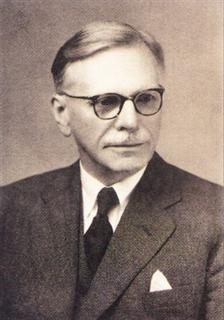
\includegraphics[height=3cm]{firth.png}
            \end{figure}
            \begin{center}
                \tiny
                J.R. Firth \\
                Lingüísta inglés \\
                1890-1960\\
            \end{center}
        \end{column}
        \begin{column}{6cm}
            \begin{itemize}
                %\pause
                \item \citeA{cabre_panorama_2003}: fundador del funcionalismo lingüístico
                \begin{itemize}
                    %\pause
                    \item Incorporó las ideas del antropólogo Mainowski quien dijo: \textit{```el lenguaje no es un sistema en sí mismo (posición estructuralista extrema) sino que evoluciona por las demandas de la sociedad y su contexto'''} (11).
                    %\pause
                    \item Se le atribuye ser el primero en estudiar colocaciones \cite{bartsch_towards_2014}
                \end{itemize}
            \end{itemize}
        \end{column}
    \end{columns}
\end{frame}


\begin{frame}{Antecedentes históricas}
    \begin{columns}
        \begin{column}{6cm}
            \begin{figure}
            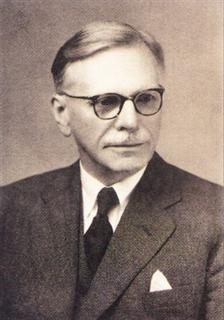
\includegraphics[height=1.8cm]{firth.png}
            \end{figure}
            \begin{center}
                \tiny
                J.R. Firth \\
                Lingüísta inglés \\
                1890-1960\\
            \end{center}
            \begin{figure}
                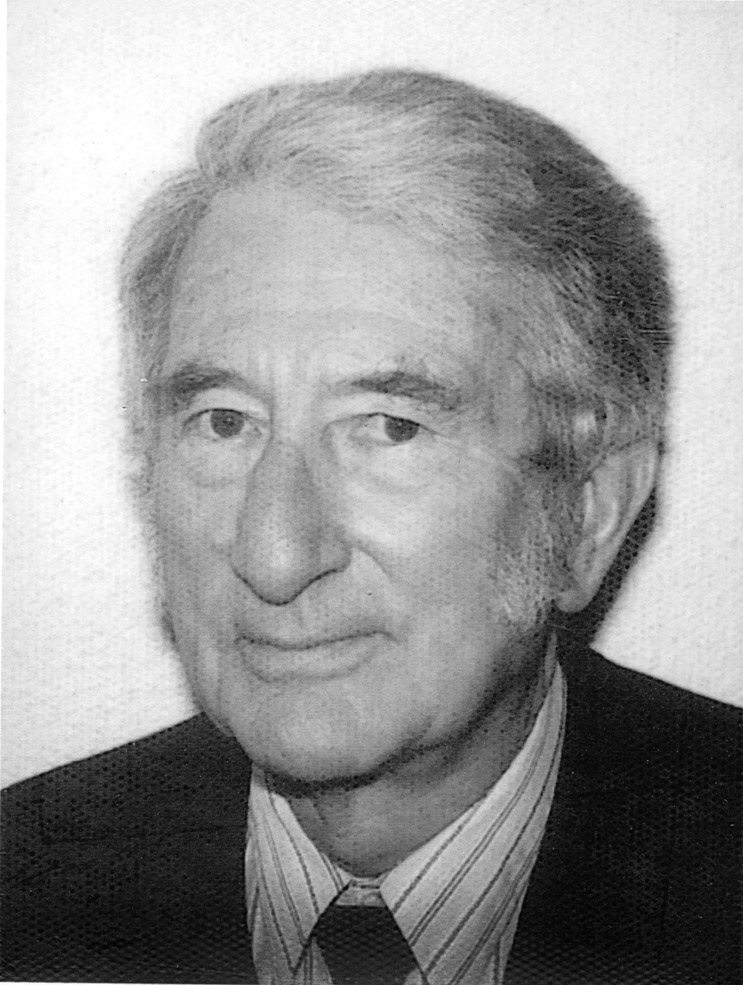
\includegraphics[height=1.8cm]{halliday.jpg}
            \end{figure}
            \begin{center}
                \tiny
                Michael Halliday \\
                Fundador de la gramática sistémico funcional \\
                1925-\\
            \end{center}
        \end{column}
        \begin{column}{6cm}
            \begin{flushleft}
            \begin{figure}
                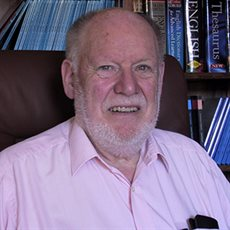
\includegraphics[height=1.8cm]{sinclair.jpg}
            \end{figure}
            \begin{center}
            \tiny
            John McHardy Sinclair \\
            Fundador de la lingüística de corpus \\
            1933-2007\\
            \end{center}
            \end{flushleft}
        \end{column}
    \end{columns}
\end{frame}


\begin{frame}{Sinclair}
    \begin{columns}
        \begin{column}{6cm}
            \begin{figure}
            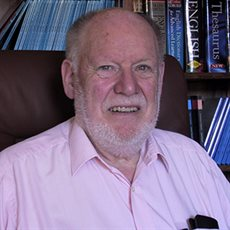
\includegraphics[height=3cm]{sinclair.jpg}
            \end{figure}
            \begin{center}
            \begin{tiny}
            John McHardy Sinclair \\
            Fundador de la lingüística de corpus \\
            1933-2007\\
            \end{tiny}
            \end{center}
        \end{column}
        \begin{column}{6cm}
            \begin{itemize}
                %\pause
                \item Fundador del proyecto \textbf{COBUILD} (Collins and Birmingham University International Language Database)
                \begin{itemize}
                    %\pause
                    \item Revolucionó la lexicógrafia \cite[p. 58]{simpson_lexicography_2011}
                \end{itemize}
                %\pause
                \item Famoso por dos principios de la lingüística de corpus
                \begin{itemize}
                    %\pause
                    \item \textit{the open choice principle}
                    \item \textit{the idiom principle}
                    \citeA{sinclair_trust_2004}
                \end{itemize}
            \end{itemize}
        \end{column}
    \end{columns}
\end{frame}

\begin{frame}{The Open Choice Principle}
    \begin{columns}
        \begin{column}{6cm}
            \begin{figure}
                \begin{turn}{270}
                % Notice a little bit of manual adjusting
                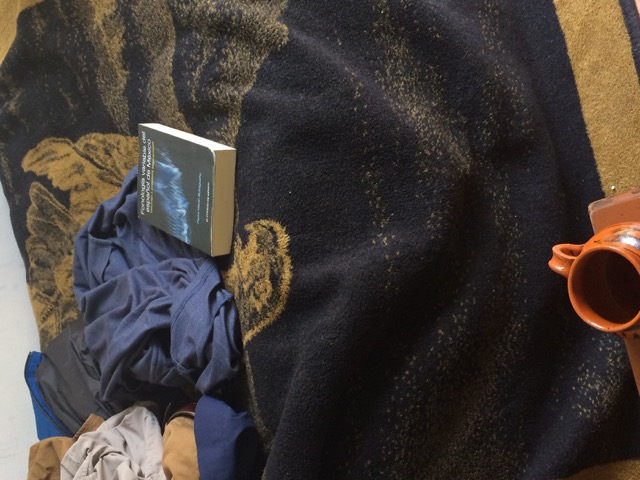
\includegraphics[height=2.0cm, width=1.6cm]{pbm.JPG}
                \end{turn}
            \end{figure}
            \begin{figure}
                \begin{turn}{270}
                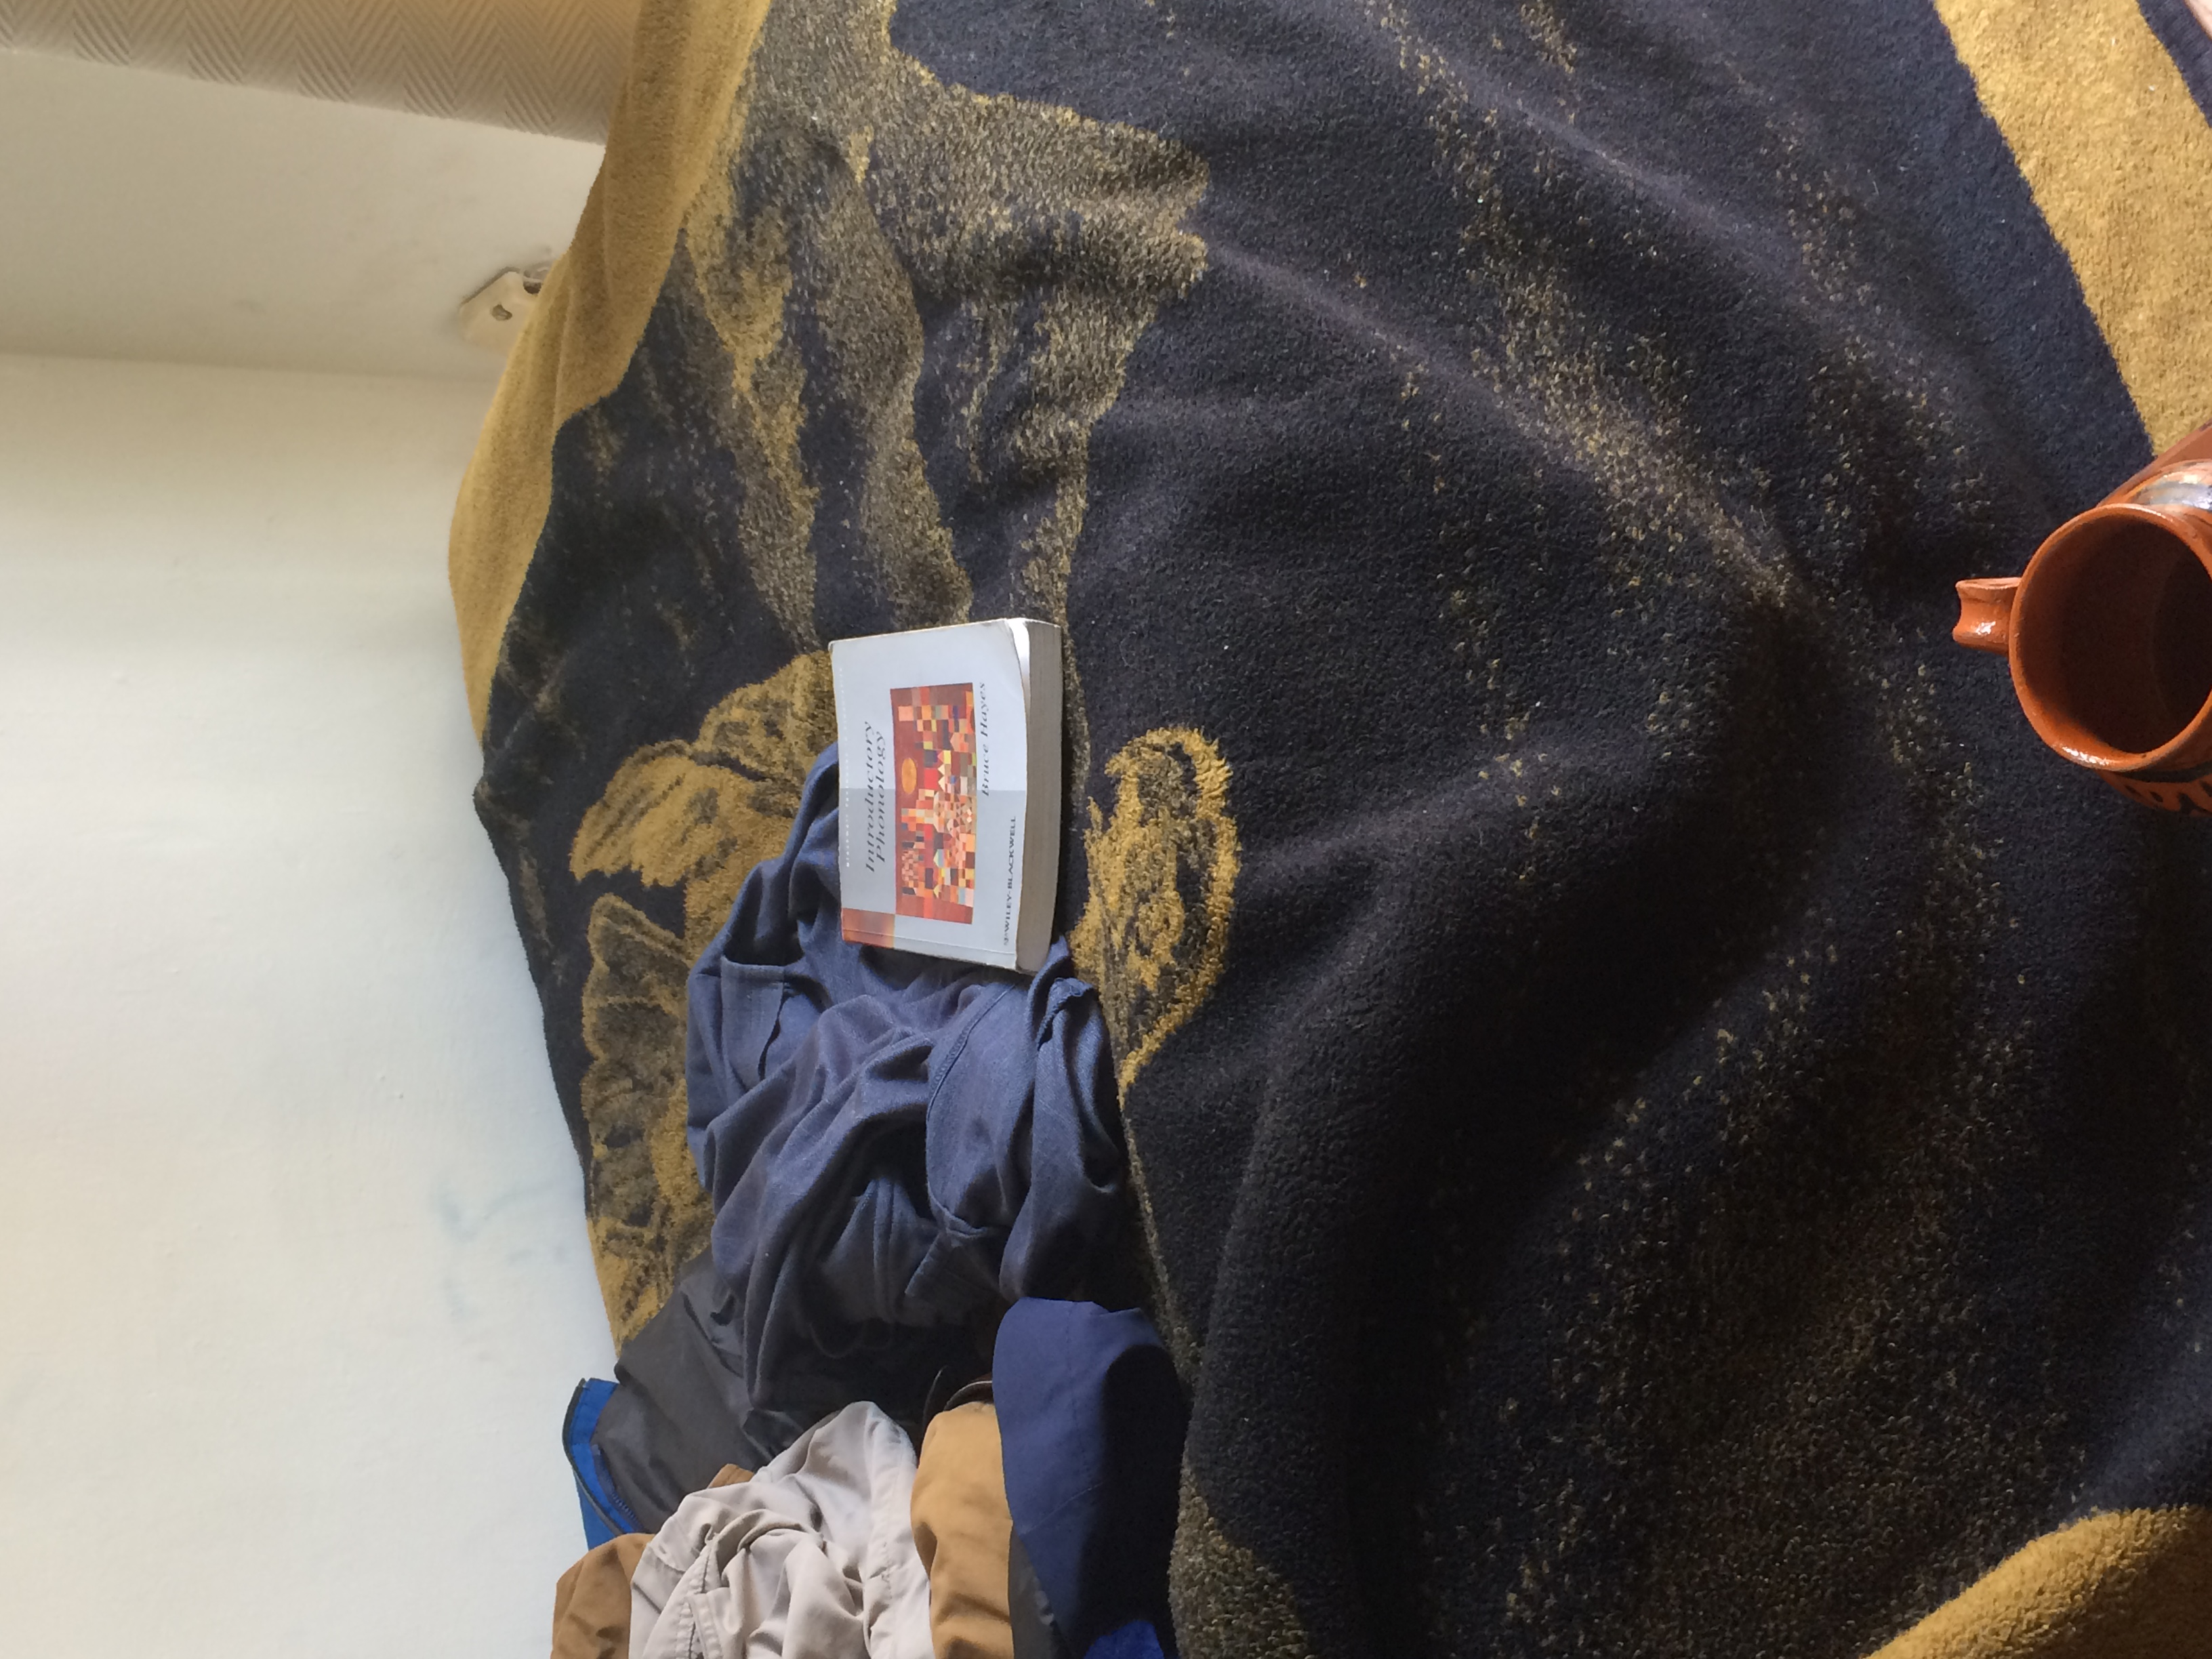
\includegraphics[height=2.0cm, width=1.6cm]{hayes.JPG}
                \end{turn}
            \end{figure}
            \begin{figure}
                \begin{turn}{270}
                
\includegraphics[height=2.0cm, width=1.6cm]{sonoro.JPG}
                \end{turn}
            \end{figure}
        \end{column}
        \begin{column}{6cm}
        \begin{itemize}
        %This vspace{} command is perfect, gets the column on the right just perfectly
        \vspace{2em}
        \item \textcolor{blue}{{[El libro de fonología variable de México]}}\textcolor{red}{\textsubscript{FN}} está sobre la cama.
        \begin{itemize}
            %\pause
            \item que fue escrito por el lingüísta X
        \end{itemize}
        %\pause
        \item \textcolor{blue}{{[El libro de fonología introductoria]}}\textcolor{red}{\textsubscript{FN}} está sobre la cama.
        \begin{itemize}
            \item que leímos para la clase de Fonética
        \end{itemize}
        \item \textcolor{blue}{{[El libro de fonología de las lenguas indígenas de México]}}\textcolor{red}{\textsubscript{FN}} está sobre la cama.
        \begin{itemize}
            \item que se publicó en el Colegio de México
        \end{itemize}
        \end{itemize}
        \end{column}
    \end{columns}
\end{frame}

\begin{frame}{Kahoot Question 1: The Idiom Principle}
    \begin{columns}
        \begin{column}{6cm}
            \begin{figure}
                \begin{turn}{270}
                % Notice a little bit of manual adjusting
                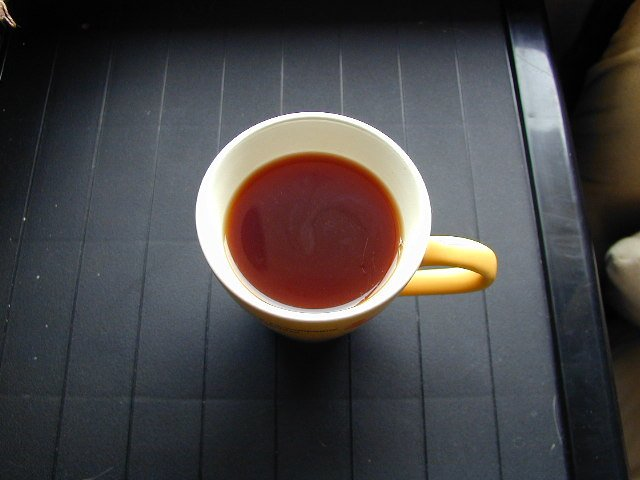
\includegraphics[height=3cm, width=3cm]{Black-tea.jpg}
                \end{turn}
            \end{figure}
        \end{column}
        \begin{column}{6cm}
        %\pause
        \begin{itemize}
            \item Words tend to co-occur, so our lexicon is really composed of 'lexical bundles'.
            \begin{itemize}
                %\pause
                \item Sinclair (39) calls these structures compound lexical items and he identifies the following component parts:
                \begin{itemize}
                    %\pause
                    \item Collocation
                    %\pause
                    \item Colligation
                    %\pause
                    \item Semantic preference
                    %\pause
                    \item Semantic Prosody
                \end{itemize}
            \end{itemize}
        %\pause
        \item Kahoot 1
        %\pause
        \item Let's run through Sinclair's analysis of the \textit{true feelings} with the Corpus of Contemporary American English
        \end{itemize}
        \end{column}
    \end{columns}
\end{frame}

\section{Aplicando la teoría de Sinclair en los corpus}

\begin{frame}{True Feelings (Sinclair's Example p.35)}
    \begin{center}
    \textbf{Let's check out \textit{True Feelings} with the Corpus of Contemporary American English}
    \end{center}
    \begin{columns}
        \begin{column}{15cm}
            \begin{itemize} 
            %\pause
            \item start with collocation: \textcolor{red}{{[true feelings]}\textsubscript{semantic core}}
            %\pause
            \item List most frequent words that occur at n-1
                \begin{itemize}
                    %\pause
                    \item \textcolor{blue}{{[poss. adj.]}\textsubscript{colligation}} + \textcolor{red}{{[true feelings]}\textsubscript{s.c.}}
                \end{itemize}
            %\pause
            \item List common verb collocations in range n-4
                \begin{itemize}
                    %\pause
                    \item \textcolor{green}{{[verb of expression]}\textsubscript{semantic preference}}+ \textcolor{blue}{{[poss. adj.]}\textsubscript{colli.}} + \textcolor{red}{{[true feelings]}\textsubscript{sc}}
                \end{itemize}   
             %\pause
             \item Use KWIC to get semantic prosody
                \begin{itemize}
                    %\pause
                    \item Semantic Prosody: Negative/Reluctance 
                \end{itemize}
                \vspace{2em}
                %\pause
                \textbf{Final Lexical Bundle:} \\
                    \textbf{{[}}{[\textcolor{green}{{[v. exp.]}\textsubscript{sem. pref.}}+ \textcolor{blue}{{[poss. adj.]}\textsubscript{colli.}} + \textcolor{red}{{[true feelings]}\textsubscript{sc}}]}\textsubscript{sem pros: neg/rel.}{]}\textbf{{]}}
            \end{itemize}
        \end{column}   
    \end{columns}
\end{frame}

\begin{frame}{Carecer - own analysis}
    \begin{center}
    \textbf{Vamos a analizar \textit{carecer} con el Corpus de Español}
    \end{center}
    \begin{columns}
        \begin{column}{15cm}
            \begin{itemize} 
            %\pause
            \item Start with colligation/collocation: \textcolor{red}{{[carecer]}\textsubscript{semantic core}} + \textcolor{blue}{{[de]}\textsubscript{colligation}}
           %\pause
           \item List frequent noun collocations occurring in the range (n + 3)
                \begin{itemize}
                    %\pause
                    \item \textcolor{red}{{[carecer]}\textsubscript{s.c}} + \textcolor{blue}{{[de]}\textsubscript{colli.}} + \textcolor{green}{{[}FN{]}\textsubscript{semantic preference: something positive}}
                \end{itemize}
            %\pause
            \item What is the semantic prosody?
                \begin{itemize}
                    \item Kahoot Question 2
                \end{itemize}
                \vspace{2em}
                %\pause
                \textbf{Final Lexical Bundle:}\\
                {[}{[}\textcolor{red}{{[carecer]}\textsubscript{s.c}} + \textcolor{blue}{{[de]}\textsubscript{colli.}} + \textcolor{green}{{[}FN{]}\textsubscript{sem pref: positive}}{]}\textsubscript{sem pros: neg./lamenting}{]}{]}
         \end{itemize}
        \end{column}   
    \end{columns}
\end{frame}

\begin{frame}
\begin{columns}
\begin{column}{4cm}
\begin{figure}
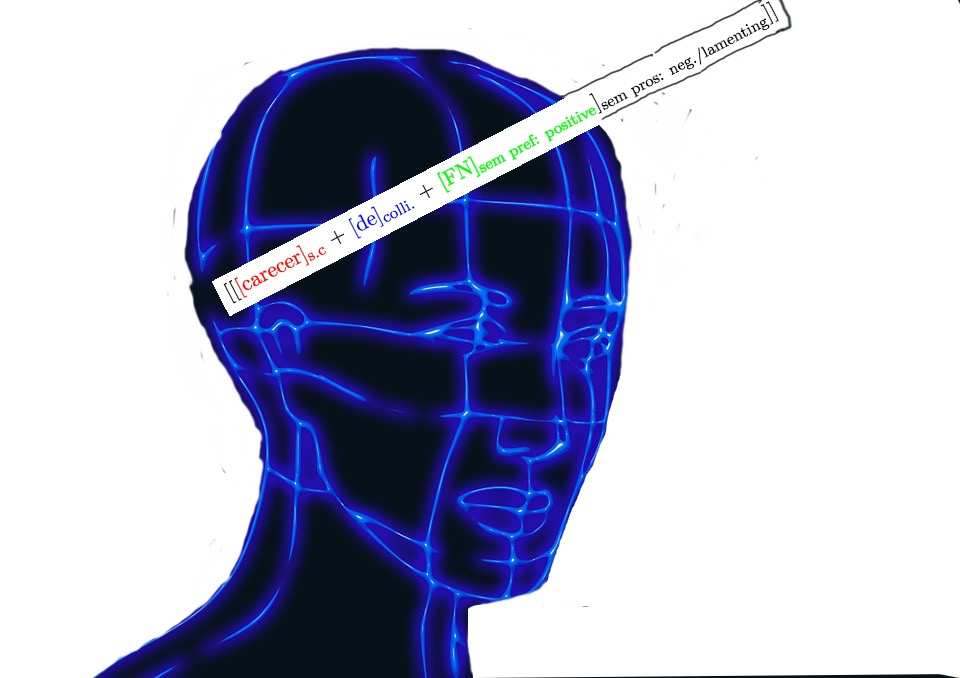
\includegraphics[height=3cm]{phrasehead.jpg}
\end{figure}
\end{column}
\begin{column}{6cm}
\begin{itemize}
%\pause
\item In academic blog post \textit{Why Chomsky was wrong about corpus linguistics} \citeA{wallis_why_2016} explains theoretical clash with Sinclair.
\begin{itemize}
%\pause
\item Chomsky = I-language (linguistic competence) \textbf{not E-language}(linguistic performance)
%\pause
\item Siclair: Build grammar from the \textbf{"bottom-up".}
\end{itemize}
%\pause
\item Today, few linguists rely on introspection and value-judgments; few applied linguistics lack theory in their analysis .
\end{itemize}
\end{column}
\end{columns}
\end{frame}


\section{The Use Of Corpora in Other Fields: Language Teaching}

\begin{frame}{Types of Corpora}

\begin{table}
\centering
\caption{Some Types of Corpora Listed By \citeA{simpson_corpus_2011}}
\label{my-label}
\begin{tabular}{ll}
\textbf{Type} & \textbf{Example}  \\ 
    %\pause
    Historical & Corpus diacrónico del español (CORDE)  \\
    %\pause
    Monitor & COCA, Corpus de Español  \\
    %\pause
    Learner & The International Corpus of Learner English  \\
    %\pause
    Parallel & Linguee.com 
\end{tabular}
\end{table}
\end{frame}

\begin{frame}{Language Teaching}
    \begin{columns}
        \begin{column}{4cm}
            \begin{figure}
                
\includegraphics[height=3cm]{lei.jpg}
                    \begin{center}
                        \begin{tiny}
                        Using Corpora for Language Learning and Teaching\\
                        \cite{liu_using_2017}
                        \end{tiny}
                    \end{center}
            \end{figure}
        \end{column}
        
        \begin{column}{6cm}
        \begin{itemize}
            %\pause
            \item \textbf{Inductive} vs. \textbf{Deductive} Corpora Use in the Classroom
        \begin{itemize}
            %\pause
            \item Inductive: Students ``discover" the language patterns for themselves, engage in deep-learning
            %\pause
            \item Deductive: Confirming or reinforcing what you already know (Come up with a small worksheet that students can fill out, completing some kind of information that they have)
        \end{itemize}
    \end{itemize}
\end{column}
\end{columns}
\end{frame}

\begin{frame}{Language Teaching - Example 1}
    \begin{columns}
        \begin{column}{6cm}
            \begin{figure}
                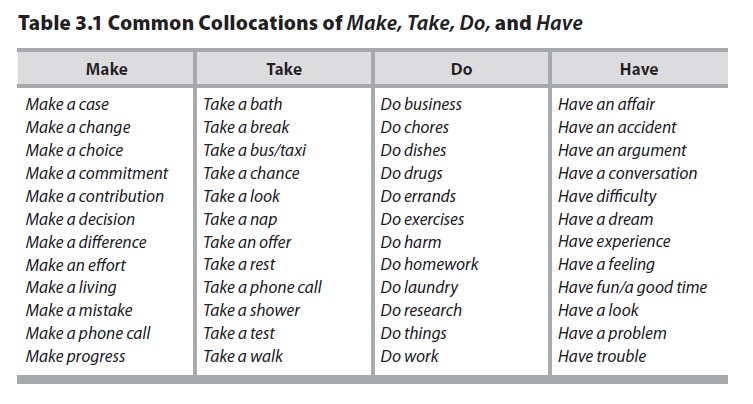
\includegraphics[height=3cm]{maketake.jpg}
                    \begin{center}
                        \begin{tiny}
                        Table reproduced from \cite[p.39]{liu_using_2017}
                        \end{tiny}
                    \end{center}
            \end{figure}
        \end{column}
        
        \begin{column}{4cm}
        \begin{itemize}
            %\pause
            \item Is it easier to \textit{make} or \textit{take} something?
            %\pause
            \item Which verb is used with routines?
            %\pause
            \item What about have? Can you replace these verbs with another verb?
        \end{itemize}
\end{column}
\end{columns}
\end{frame}


%%%%Make sure to get reference
\begin{frame}{Language Teaching - Example 2}
    \begin{itemize}
        %\pause
        \item According to \cite{cowan_teachers_2008} some phrasal verbs are separable: \textit{set up, hand in, look up}
        \begin{itemize}
        %\pause
        \item I set up {[}the machine{]}\textsubscript{NP}
        %\pause
        \item I set {[}the machine{]}\textsubscript{NP} up 
        \end{itemize}
        %\pause
        \item What can the following data tell us about separable phrasal verbs?
    \end{itemize}
        \begin{columns}
        \begin{column}{5cm}
        \begin{table}
    \centering
    \caption{set up + NP}
     \scalebox{0.75}{
    \begin{tabular}{|l|l|l|}
        \hline
        Rank & Example & Hits \\ \hline
        1 & SET UP THE TENT & 24 \\
        2 & SET UP THE SYSTEM & 20 \\
        3 & SET UP THE EQUIPMENT & 19 \\
        4 & SET UP THE MEETING & 18 \\
        5 & SET UP THE CAMERA & 17 \\
        6 & SET UP THE TELESCOPE & 10 \\
        7 & SET UP THE CONDITIONS & 9 \\
        8 & SET UP THE COURSE & 9 \\
        9 & SET UP THE GAME & 9 \\
        \hline
    \end{tabular}}
    \end{table}
        
        \end{column}
        \begin{column}{5cm}
        \begin{table}
        \centering
    \caption{set (NP) up}
        \scalebox{0.8}{
    \begin{tabular}{|l|l|l|}
        \hline
        Rank & Example & Hits \\ \hline
        1 & SET IT UP & 618 \\
        2 & SET ME UP & 241 \\
        3 & SET HIM UP & 235 \\
        4 & SET THEM UP & 194 \\
        5 & SET YOU UP & 185 \\
        6 & SET HER UP & 114 \\
        7 & SET HIMSELF UP & 110 \\
        8 & SET US UP & 87 \\
        9 & SET YOURSELF UP & 84 \\
        \hline
    \end{tabular}}
\end{table}
    
    \end{column}
    \end{columns}

\end{frame}

\begin{frame}{Example 2 - All Data}

\begin{columns}
        \begin{column}{5cm}
        \begin{table}
    \centering
    \caption{set up + NP}
     \scalebox{0.5}{
    \begin{tabular}{|l|l|l|}
        \hline
        Rank & Example & Hits \\ \hline
        1 & SET UP THE TENT & 24 \\
        2 & SET UP THE SYSTEM & 20 \\
        3 & SET UP THE EQUIPMENT & 19 \\
        4 & SET UP THE MEETING & 18 \\
        5 & SET UP THE CAMERA & 17 \\
        6 & SET UP THE TELESCOPE & 10 \\
        7 & SET UP THE CONDITIONS & 9 \\
        8 & SET UP THE COURSE & 9 \\
        9 & SET UP THE GAME & 9 \\
        \hline
    \end{tabular}}
    \end{table}
        
        \begin{table}
         \centering
    \caption{set + NP + up}
    \scalebox{.5}{
    \begin{tabular}{|l|l|l|}
        \hline
        Rank & Example & Hits \\ \hline
        1 & SET THE CAMERA UP & 7 \\
        2 & SET THE LEVEL UP & 3 \\
        3 & SET THE COURSE UP & 3 \\
        4 & SET THE BATHROOM UP & 2 \\
        5 & SET THE BOAT UP & 2 \\
        6 & SET THE CONTRAPTION UP & 2 \\
        7 & SET THE COMPUTER UP & 2 \\
        8 & SET THE COMPANY UP & 2 \\
        9 & SET THE DOCTOR UP & 2 \\
        \hline
    \end{tabular}}
\end{table}
              
        \end{column}
        \begin{column}{5cm}
        \begin{table}
        \centering
    \caption{set + prn. + up}
        \scalebox{0.5}{
    \begin{tabular}{|l|l|l|}
        \hline
        Rank & Example & Hits \\ \hline
        1 & SET IT UP & 618 \\
        2 & SET ME UP & 241 \\
        3 & SET HIM UP & 235 \\
        4 & SET THEM UP & 194 \\
        5 & SET YOU UP & 185 \\
        6 & SET HER UP & 114 \\
        7 & SET HIMSELF UP & 110 \\
        8 & SET US UP & 87 \\
        9 & SET YOURSELF UP & 84 \\
        \hline
    \end{tabular}}
\end{table}
        \begin{table}
        \centering
    \caption{set + up + prn.}
    \scalebox{.5}{
    \begin{tabular}{|l|l|l|}
        \hline
        Rank & Example & Hits \\ \hline
        1 & SET UP SOMETHING & 21 \\
        2 & SET UP EVERYTHING & 14 \\
        3 & SET UP YOU & * \\
        4 & SET UP HIMSELF & * \\
        5 & SET UP ONE & * \\
        6 & SET UP IT & * \\
        7 & SET UP I & * \\
        8 & SET UP WE & * \\
        9 & SET UP ANYTHING & * \\
        \hline
    \end{tabular}}
\end{table}
    \end{column}
    \end{columns}

\end{frame}

\section{AntConc}

\begin{frame}{Building a local corpus}
\begin{itemize}
%\pause
\item You want your corpus to be representative
%\pause
\item Corpus can be scientific or practical
%\pause
\item Differences between Online and Offline Corpus

\begin{table}
\centering
\caption{Pros and Cons of Using a Local Corpus}
\label{pros_cons}
\scalebox{.8}{
\begin{tabular}{ll}
\textbf{Pros} & \textbf{Cons} \\ 
Flexibility, complex queries & Requires technical skill to preprocess data:  \\
Control over data & Website owns data  \\
Free & Pay for Premium Features \\
\end{tabular}}
\end{table}



\end{itemize}


\end{frame}


\begin{frame}{Software from Laurence Anthony}
    \begin{columns}
        \begin{column}{6cm}
            \begin{figure}
            
\includegraphics[height=1.8cm]{AntFileConverter.png}
            \end{figure}
            \begin{center}
                \tiny
                AntFileConverter \\
            \end{center}
            \begin{figure}
                
\includegraphics[height=1.8cm]{AntWordProfiler.png}
            \end{figure}
            \begin{center}
                \tiny
                AntWordProfiler
            \end{center}
        \end{column}
        \begin{column}{6cm}
            \begin{flushleft}
            \begin{figure}
                
\includegraphics[height=1.8cm]{AntConc.png}
            \end{figure}
            \begin{center}
            \tiny
            AntConc
            \end{center}
            \end{flushleft}
        \end{column}
    \end{columns}
\end{frame}






\begin{frame}
\begin{itemize}
\item Let's create our own corpus from PDF Files
\item And see a practical application of AntConc
\end{itemize}
\end{frame}
    
\section{References}

\begin{frame}[allowframebreaks]{Bibliography}
\bibliographystyle{apacite}

\bibliography{Zotero}

\end{frame}
\end{document}
